\documentclass[9pt]{beamer}
\beamertemplatenavigationsymbolsempty

\usepackage{subfig}

\definecolor{TriangleColor}{RGB}{255,170,128} % Soft Coral
\definecolor{LineColor}{RGB}{0,128,128}        % Darker Blue/Teal
\definecolor{VertexColor}{RGB}{255,255,128}    % Light Yellow

\usepackage{etex, tikz, array, graphics, xspace, relsize, multirow}
\usepackage[export]{adjustbox}
\usepackage{ulem}

\usetikzlibrary{arrows}
\usetikzlibrary{tikzmark}

% Frame / section / subtitle title colors
\setbeamercolor{frametitle}{fg=LineColor}
\setbeamercolor{title}{fg=LineColor}
\setbeamercolor{subtitle}{fg=LineColor}

\renewenvironment{theorem}[1][]{\textcolor{LineColor}{\textbf{Theorem #1}} }{}
\renewenvironment{definition}[1][]{\textcolor{LineColor}{\textbf{Definition #1}} }{}

\usepackage{enumitem}
\setlist[itemize]{label=\textcolor{LineColor}{\textbullet}}
\PassOptionsToPackage{hyperfootnotes=false}{hyperref}
\usepackage{bbding}
\usepackage{pdflscape}
\usepackage{rotating}\setlength{\rotFPtop}{0pt plus 1fil}
\overfullrule=1ex

% Tikz drawing
\usetikzlibrary{arrows.meta}
\usepackage{tcolorbox}
\usetikzlibrary{matrix,fit,positioning,shapes.geometric,patterns,backgrounds}
\usetikzlibrary{decorations.pathreplacing,decorations.markings,calc}
\tikzset{>=stealth'}

\usepackage[draft=false]{minted}
\usemintedstyle{default}
\setminted{fontsize=\scriptsize, frame=single, framesep=2mm}

\usepackage{booktabs}
\usepackage{amsmath}

% Names
\newcommand\Julia{\texttt{Julia}\xspace}
\newcommand\OSCAR{\texttt{OSCAR}\xspace}
\newcommand\polymake{\texttt{polymake}\xspace}
\newcommand\Macaulay{\texttt{Macaulay2}\xspace}
\newcommand{\mrdi}{\texttt{mrdi}\xspace}

% Number sets / caligraphics from the paper
\newcommand{\cc}{\mathbb{C}}
\newcommand{\rr}{\mathbb{R}}
\newcommand{\qq}{\mathbb{Q}}
\newcommand{\zz}{\mathbb{Z}}
\newcommand{\pp}{\mathbb{P}}
\newcommand{\PP}{\mathbb{P}}
\newcommand{\cm}{\mathcal{M}}
\newcommand{\ct}{\mathcal{T}}
\newcommand{\pd}{\mathrm{PD}}
\newcommand{\indep}{\mathrel{\text{$\perp\mkern-10mu\perp$}}}
\newcommand{\sym}{\mathrm{sym}}

\usenavigationsymbolstemplate{}

\author[Antony Della Vecchia]{Tobias Boege, \textbf{Antony Della Vecchia},\\ Marina Garrote L\'opez, Benjamin Hollering}
\title{Phylogenetic models, Data Structures and Tools}
\institute[]{TU Berlin}
\date{ICMS 2026-07-22}

% Itemize that spreads its items to fill the frame vertically
\newenvironment{fillitemize}
  {\vspace{\fill}\begin{itemize}\setlength{\itemsep}{\fill}}
  {\end{itemize}\vspace{\fill}}

% ---- Reusable tikz: rooted phylogenetic tree (3 leaves) with branch lengths ----
% Binary topology r->{1, u}, u->{2,3}; edges have visibly different lengths,
% labelled with branch lengths t_i.
\newcommand{\phylotree}[1][0.9]{%
  \begin{tikzpicture}[scale=#1, every node/.append style={transform shape},
    inner/.style={circle, draw=LineColor, thick, fill=TriangleColor, minimum size=6mm, font=\small},
    leaf/.style={circle, draw=LineColor, thick, fill=VertexColor, minimum size=7mm, font=\small\bfseries},
    blen/.style={font=\scriptsize, fill=white, inner sep=1pt},
    every edge/.append style={draw=LineColor, thick}]
    \node[inner] (r) at (0,3.2)   {$r$};
    \node[inner] (u) at (1.1,1.5) {};
    \node[leaf] (l1) at (-2.2,0)  {1};
    \node[leaf] (l2) at (0.4,0)   {2};
    \node[leaf] (l3) at (2.4,0)   {3};
    \draw[->] (r) -- (l1) node[midway, blen, left=1pt]{$M_1$};
    \draw[->] (r) -- (u)  node[midway, blen, right=1pt]{$M_2$};
    \draw[->] (u) -- (l2) node[midway, blen, left=1pt]{$M_3$};
    \draw[->] (u) -- (l3) node[midway, blen, right=1pt]{$M_4$};
  \end{tikzpicture}%
}

% ---- Reusable tikz: star tree (1 internal node, 3 leaves) ----
\newcommand{\startree}[1][0.9]{%
  \begin{tikzpicture}[scale=#1, every node/.append style={transform shape},
    inner/.style={circle, draw=LineColor, thick, fill=TriangleColor, minimum size=6mm, font=\small},
    leaf/.style={circle, draw=LineColor, thick, fill=VertexColor, minimum size=7mm, font=\small\bfseries},
    blen/.style={font=\scriptsize, fill=white, inner sep=1pt},
    every edge/.append style={draw=LineColor, thick}]
    \node[inner] (r) at (0,1.8)   {$r$};
    \node[leaf] (l1) at (-2.2,0)  {1};
    \node[leaf] (l2) at (0,0)     {2};
    \node[leaf] (l3) at (2.2,0)   {3};
    \draw[->] (r) -- (l1) node[midway, blen, left=1pt]{$M_1$};
    \draw[->] (r) -- (l2) node[midway, blen, right=1pt]{$M_2$};
    \draw[->] (r) -- (l3) node[midway, blen, right=1pt]{$M_3$};
  \end{tikzpicture}%
}

% ---- Reusable tikz: 3-leaf sunlet network (central 3-cycle + pendants) ----
\newcommand{\sunletnet}[1][0.9]{%
  \begin{tikzpicture}[scale=#1, every node/.append style={transform shape},
    inner/.style={circle, draw=LineColor, thick, fill=TriangleColor, minimum size=6mm, font=\small},
    hyb/.style={circle, draw=red, very thick, fill=TriangleColor, minimum size=6mm, font=\small},
    leaf/.style={circle, draw=LineColor, thick, fill=VertexColor, minimum size=7mm, font=\small\bfseries},
    every edge/.append style={draw=LineColor, thick}]
    \node[inner] (n5) at (-1,1.6) {5};
    \node[inner] (n6) at (1,1.6)  {6};
    \node[hyb]   (n4) at (0,0.3)  {4};
    \node[leaf] (l2) at (-2.4,2.4) {2};
    \node[leaf] (l3) at (2.4,2.4)  {3};
    \node[leaf] (l1) at (0,-1.4)   {1};
    \draw[->] (n5) -- (n6);
    \draw[->] (n5) -- (n4);
    \draw[->] (n6) -- (n4);
    \draw[->] (n5) -- (l2);
    \draw[->] (n6) -- (l3);
    \draw[->] (n4) -- (l1);
  \end{tikzpicture}%
}

% ---- Reusable tikz: 4-leaf sunlet network (3-node path + hybrid) ----
\newcommand{\sunletnetfour}[1][0.9]{%
  \begin{tikzpicture}[scale=#1, every node/.append style={transform shape},
    inner/.style={circle, draw=LineColor, thick, fill=TriangleColor, minimum size=6mm, font=\small},
    hyb/.style={circle, draw=red, very thick, fill=TriangleColor, minimum size=6mm, font=\small},
    leaf/.style={circle, draw=LineColor, thick, fill=VertexColor, minimum size=7mm, font=\small\bfseries},
    every edge/.append style={draw=LineColor, thick}]
    \node[inner] (n5) at (-2.2,2.2) {5};
    \node[inner] (n6) at (0,2.8)    {6};
    \node[inner] (n7) at (2.2,2.2)  {7};
    \node[hyb]   (n4) at (0,0.4)    {4};
    \node[leaf] (l1) at (-2.8,0.4)  {1};
    \node[leaf] (l2) at (0,4.0)     {2};
    \node[leaf] (l3) at (2.8,0.4)   {3};
    \node[leaf] (l4) at (0,-0.9)    {4};
    \draw[->] (n5) -- (n6);
    \draw[->] (n6) -- (n7);
    \draw[->] (n5) -- (n4);
    \draw[->] (n7) -- (n4);
    \draw[->] (n5) -- (l1);
    \draw[->] (n6) -- (l2);
    \draw[->] (n7) -- (l3);
    \draw[->] (n4) -- (l4);
  \end{tikzpicture}%
}

\begin{document}

%% ---------------------------------------------------------------- Title
\begin{frame}[plain]
  \vfill
  \begin{columns}[c]
    \begin{column}{0.55\textwidth}
      \raggedright
      {\usebeamercolor[fg]{title}\usebeamerfont{title}\inserttitle\par}
      \bigskip
      {\usebeamerfont{author}\insertauthor\par}
      \medskip
      {\usebeamercolor[fg]{institute}\usebeamerfont{institute}\insertinstitute\par}
      \smallskip
      {\usebeamerfont{date}\insertdate\par}
    \end{column}
    \begin{column}{0.45\textwidth}
      \centering
      \phylotree[0.7]
    \end{column}
  \end{columns}
  \vfill
  \noindent
  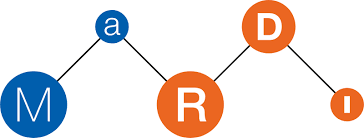
\includegraphics[width=2.2cm]{images/mardi-logo.png}%
  \hfill
  
\includegraphics[width=2.2cm]{images/oscar.pdf}
\end{frame}

%% ---------------------------------------------------------------- Overview
\begin{frame}{Overview}
  \begin{itemize}[itemsep=2em]
  \item \textbf{Background} --- graphical models, algebraic phylogenetics.
  \item \textbf{Implementation} --- data structures and tools for working with these models in \OSCAR.
  \item \textbf{Ongoing work}.
  \end{itemize}
\end{frame}

%% ---------------------------------------------------------------- 1b. General setup
\begin{frame}{Graphical Models}
  \vspace{-4em}
  \begin{itemize}
  \item Fix a graph $G$.
  \item $\Theta \subseteq \rr^d$  a semi algebraic set of parameters attached to $G$.
  \item  $\Delta$ the space of \textbf{all distributions} on the observed variables.
    \end{itemize}
  \bigskip

  \begin{center}
    \Large $\varphi : \Theta \to \cm_G \subseteq \Delta$
  \end{center}
  \vspace{4em}
  \pause
  \begin{itemize}[itemsep=1.5em]
  \item Want to understand invariants that come from the Graph. \pause
  \item In general many different types of graphs and statistical models. \pause
  \item Use commutative algebra to understand $\overline{\cm_G} = \overline{\varphi(\Theta)}$.
  \end{itemize}
\end{frame}

%% ---------------------------------------------------------------- 2. Recap
\begin{frame}{Algebraic Phylogenetics}
  \begin{columns}[c]
    \begin{column}{0.45\textwidth}
      \centering
      \phylotree[0.7]
    \end{column}
    \begin{column}{0.55\textwidth}
      \begin{itemize}
      \item Markov property: $X_v$ depends only on ancestor and transition matrix $M_e$ on that edge. \pause
      \item Want to find invariants in terms of the observables at the leaves. \pause
      \item Hidden internal nodes $\Rightarrow$ marginalize:
        \[
          p_{i_1\dots i_n} =\!\!
          \sum_{\substack{x_v,\, v\text{ internal}}}\!\!
          \pi(x_r)\!\!\prod_{u\to v}\!\! M_e(x_u,x_v).
        \] \pause
      \item Use invariants of the leaves to distinguish between topologies. \pause
      \end{itemize}

    \end{column}
  \end{columns}
\end{frame}


%% ---------------------------------------------------------------- 4. Why Julia
\begin{frame}[fragile]{The General Graphical Model Framework}
\begin{minted}{julia}
abstract type GraphicalModel{T <: AbstractGraph, L <: Union{NamedTuple, Nothing}} end
\end{minted}
  \pause
  \begin{center}
    \Large $\varphi^{*} : S \to R$
  \end{center}
  Given implementations for

  \begin{itemize}
  \item \texttt{model\_ring} (returns  $S$ coordinate ring of $\cm$)
  \item \texttt{parameter\_ring} (returns $R$ coordinate ring of $\Theta$)
  \item \texttt{parametrization} (returns $\varphi^{*}$)
  \end{itemize}
  \vspace{2em}
  We can write a generic \texttt{vanishing\_ideal} implementation. \pause
  \begin{itemize}
  \item Set up the ideal $\langle s_i - \varphi^{*}(s_i) : s_i \in S \rangle$ for each generator $s_i$ of the model ring $S$,
  \item then eliminate the variables of the parameter ring $R$.
  \end{itemize}

\end{frame}

\begin{frame}[fragile]{Constructing a \texttt{PhylogeneticModel}}
\begin{minted}{julia}
abstract type GraphicalModel{T <: AbstractGraph, L <: Union{NamedTuple, Nothing}} end

struct PhylogeneticModel{T, L, M, R} <: GraphicalModel{T, L}
    graph::T
    labelings::L
    transition_matrices_structure::Matrix{M}
    root_distribution::Vector{R}
    n_states::Int
end
\end{minted}
  \pause
Multiple ways to construct models
\begin{minted}{julia}
julia> M = [:a :b; :b :a];
julia> phylo_t = phylogenetic_tree("((H:3,(C:1,B:1):2):1,G:4);");
julia> PM1 = phylogenetic_model(phylo_t, M);
julia> typeof(PM1)
PhylogeneticModel{PhylogeneticTree{QQFieldElem}, ...}

julia> G = graph_from_edges(Directed,[[5,1], [6,5], [7,6], [7,8],
                                       [8,5], [6,2], [7,3], [8,4]]);
julia> PM2 = phylogenetic_model(G, M);
julia> typeof(PM2)
PhylogeneticModel{PhylogeneticNetwork{1, 1}, ... }
\end{minted}

\end{frame}



%% ---------------------------------------------------------------- 6. Classical models
\begin{frame}{Classical Biological Models}
  Common \textbf{linear constraints} on $\Theta$:
  \bigskip

  \[
    \underbrace{\begin{pmatrix} a&b&b&b\\ b&a&b&b\\ b&b&a&b\\ b&b&b&a\end{pmatrix}}_{\text{Jukes--Cantor}}
    \quad
    \underbrace{\begin{pmatrix} a&b&c&b\\ b&a&b&c\\ c&b&a&b\\ b&c&b&a\end{pmatrix}}_{\text{Kimura 2}}
    \quad
    \underbrace{\begin{pmatrix} a&b&c&d\\ b&a&d&c\\ c&d&a&b\\ d&c&b&a\end{pmatrix}}_{\text{Kimura 3}}
  \]
  \bigskip
  \pause

  Available in \OSCAR:
  \begin{itemize}
  \item group-based: \texttt{jukes\_cantor\_model}, \texttt{kimura2\_model},
    \texttt{kimura3\_model};
  \item \texttt{general\_markov\_model}, \texttt{general\_time\_reversible\_model}.
  \end{itemize}
\end{frame}

%% ---------------------------------------------------------------- 7. Group-based / Fourier
\begin{frame}[fragile]{Group-Based Models: Fourier $\Rightarrow$ Toric}
  \textbf{Fourier transform} diagonalizes every transition matrix.
  \bigskip

  \begin{itemize}
  \item Probability coords $p$ $\longrightarrow$ \textbf{Fourier coords} $q$.
  \item Parametrization $\to$ \textbf{monomial map}.
  \item $\Rightarrow$ \textbf{toric variety} --- uses \texttt{4ti2} to first find Markov basis.
  \end{itemize}
  \pause
  \medskip
\begin{minted}{julia}
julia> T = graph_from_edges(Directed, [[1, 2], [1, 3], [1, 4]]);
julia> GM = jukes_cantor_model(T)
Group-based phylogenetic model on a tree with 3 leaves and 3 edges 
  with root distribution [1//4, 1//4, 1//4, 1//4], 
    transition matrices of the form 
   [:a :b :b :b;
    :b :a :b :b;
    :b :b :a :b;
    :b :b :b :a]
  and fourier parameters of the form [:x, :y, :y, :y].

julia> vanishing_ideal(GM)
Ideal generated by
  -q[2,3,4]^2*q[1,1,1] + q[2,2,1]*q[2,1,2]*q[1,2,2]

julia> PM = phylogenetic_model(GM)
Phylogenetic model on a tree with 3 leaves and 3 edges 
   ...
julia> vanishing_ideal(PM)
Ideal generated by
  2*p[1,2,3]^3 - p[1,2,3]^2*p[1,2,2] - p[1,2,3]^2*p[1,2,1] - p[1,2,3]^2*p[1,1,2] +
p[1,2,3]^2*p[1,1,1] - p[1,2,3]*p[1,2,2]^2 - p[1,2,3]*p[1,2,1]^2 - p[1,2,3]*p[1,1,2]^2 +
p[1,2,3]*p[1,1,1]  ^2 + p[1,2,2]^2*p[1,2,1] + p[1,2,2]^2*p[1,1,2] + ...
\end{minted}
\end{frame}

%% ---------------------------------------------------------------- 8b. mrdi file format
\begin{frame}[fragile]{The \mrdi File Format [DV-Joswig-Lorenz 24]}
  \begin{tcolorbox}[]
    \begin{itemize}
    \item Based on JSON (Human readable).
    \item Generalizes ideas from the \texttt{polymake} format to algebraic data. 
    \item First version developed using \OSCAR. 
    \item Implementations for other systems like \Macaulay, \texttt{Magma} and \texttt{SageMath} 
    \item All types in the Algebraic Statistic section of \OSCAR can be stored using the format. 
    \end{itemize}
  \end{tcolorbox}
\end{frame}

%% ---------------------------------------------------------------- 9. Implicitization
\begin{frame}[fragile]{Multigraded Implicitization [Cummings-Hollering 26]}
  \textbf{Problem:} Generators of vanishing ideals can become very difficult to compute (Gr\"obner basis).
  \pause
  \bigskip
  
  Ideal is homogeneous in a \textbf{multigrading}, this provides an alternative to finding generators up to a given degree.
\begin{minted}{julia}
julia> M = kimura3_model(N1);          
julia> phi = parametrization(M);       
julia> comps = components_of_kernel(3, phi); 
\end{minted}
  \pause
  \begin{columns}[c]
    \begin{column}{0.52\textwidth}
      \centering\footnotesize
      \begin{tabular}{ccrr}
        \toprule
        Leaves & Deg & \Macaulay (s) & \OSCAR (s)\\
        \midrule
        4 & 2 & 0.472 & 0.050\\
        4 & 3 & 117   & 1.06\\
        5 & 2 & 329   & 0.951\\
        5 & 3 & ---   & 372\\
        \bottomrule
      \end{tabular}\\[0.3em]
      {\scriptsize Kimura 3 on sunlet networks.}
    \end{column}
    \begin{column}{0.48\textwidth}
      \centering
      \sunletnetfour[0.7]\\[0.3em]
      {\footnotesize 4-leaf sunlet network}
    \end{column}
  \end{columns}
\end{frame}

%% ---------------------------------------------------------------- 10b. Parallel results
\begin{frame}{Parallel Computation}
  \begin{columns}[c]
    \begin{column}{0.62\textwidth}
      \textbf{Parallel}:
      \begin{itemize}[itemsep=1.5em]
      \item \texttt{OSCAR} has support for multi process computations
      \item degree-5 general Markov, 3-leaf tree
      \item 32 processes, \texttt{150\,GB};
      \item $< 3$ hours vs.  $>24$ hours (serial).
      \item Results available on Zenodo \url{https://zenodo.org/records/18312720}
      \end{itemize}
    \end{column}
    \begin{column}{0.38\textwidth}
      \centering
      \startree[0.6]\\[0.3em]
      {\footnotesize $3$-leaf tree}
    \end{column}
  \end{columns}
\end{frame}

%% ---------------------------------------------------------------- 11. Serialization + DB
\begin{frame}[fragile]{Ongoing work}
  Results outlive the computation --- and the software.
  \begin{itemize}
  \item \OSCAR types $\to$ \mrdi format (JSON-based).
  \item \mrdi files $\to$ \textbf{MongoDB} database: \texttt{OscarDB}.
  \item All phylo models from \url{https://algebraicphylogenetics.org}.
  \item Plans to provide tighter integration,
  \item and expand to include networks and other model types.
  \end{itemize}
  \pause
  \vfill
  \begin{center}\Large Thank you!\end{center}
\end{frame}

\end{document}
